% latex $fileNameWithoutExt; dvisvgm $fileNameWithoutExt --bbox=papersize --font-form=ttf --precision=3 --optimize=collapse-groups,group-attributes,simplify-text,simplify-transform
\documentclass[tikz, border=2mm]{standalone}
\begin{document}
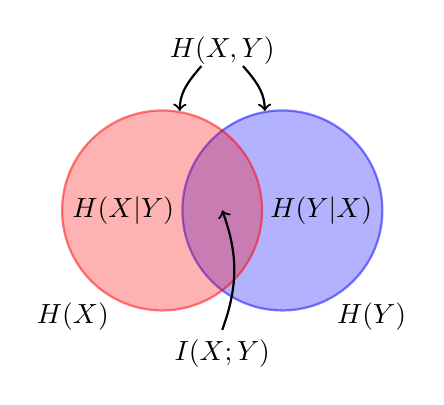
\begin{tikzpicture}
  \tikzstyle{set}=[
    circle,
    thick,
    opacity = .5,
    fill opacity = .3,
  ]
  \tikzstyle{arrow}=[{_[sep=-4px]}->, thick, opacity=1]
  \def\r{25px}
  \def\rc{36px}
  \def\circley{(-30:\r) circle (\rc)}
  \def\circlex{(-150:\r) circle (\rc)}

  \filldraw[set, blue] \circley node[set, minimum size=2*\rc] (y) {};
  \filldraw[set, red] \circlex node[set, minimum size=2*\rc] (x) {};
  \node at ([shift={(-50:50px)}]y) {$H(Y)$};
  \node at ([shift={(-130:50px)}]x) {$H(X)$};
  \node at ([shift={(0:14px)}]y) {$H(Y|X)$};
  \node at ([shift={(0:-14px)}]x) {$H(X|Y)$};
  \node (j) at (0,45px) {$H(X,Y)$};
  \draw[arrow] (j.-140) to [bend right=20] (x.80);
  \draw[arrow] (j.-40) to [bend left=20] (y.100);
  \node (i) at (0,-64px) {$I(X;Y)$};
  \draw[arrow, ->] (i.90) to [bend right=20] (0,-\r/2);
\end{tikzpicture}
\end{document}
